\documentclass[journal,10pt]{IEEEtran} % 1 page
% \documentclass[12pt,a4paper]{article} % 2.3 pages
\usepackage[utf8]{inputenc}
\usepackage{todonotes}
\usepackage{caption}

%opening
\title{AI Robot - preliminary report}
\author{Nikolaj Iversen, Matthias Harald Hessels}

\begin{document}

\maketitle

\begin{abstract}
In this paper a short description of the design choices of the Sokoban robot are defined and explained.
The robot is built using a lego mindstorm kit and the diamonds the robot has to push in the Sokoban game are tomato cans.
The Sokoban solver is not a part of the robot and the robot will receive a text file with a string of moves from the perspective of the player of the Sokoban game.
\end{abstract}

% Note that keywords are not normally used for peerreview papers.
\begin{IEEEkeywords}
Sokoban, Lego robot, Design Choices.
\end{IEEEkeywords}


\section{Behaviours}
% The AI paradigm used for this robot is a behaviour based control system.
The control system of the robot will is a reactionary control system, meaning that the robot should consist of small  simple components that react on an input rather than interpreting the world.
This is a good strategy because it allows for a lot of simple components to be tested individually and then have them brought together.
This means that the status of the robot is always known as a component is considered finished when it is working on its own.

The behaviours are split into two parts.
The first part is the robot moves. 
The robot moves governs the motors. 
The robot should be able to follow a line, the robot should be able to turn and the robot should be able to follow a line in reverse.
These are all typical reactionary modules as the robot reads on sensor values and directly outputs to the motors.
Calling a move forward function will result in the robot moves forward until it meets an intersection, thus knowing that the robot has moved forward one field.

\begin{table}[h!]
\centering
 \begin{tabular}{|l|}
  \hline
  Move set: \\
  \hline
   Turn left 90$^{\circ}$ \\
   Turn right 90$^{\circ}$\\
   Follow line forwards\\
   Follow line backwards\\
   Detect intersection \\
   \hline
 \end{tabular}
\caption{Moveset of the robot}
\label{tab:movset}
\end{table}

The moveset seen in Table \ref{tab:movset} are combined in order to make the functions needed for the robot to manoeuvre the map.

The second part is the compass function.
Since the solution to a Sokoban map is a series of moves done from the players perspective, the robot should be able to navigate the map.
The compass function governs the robot moves.
Keeping track of the map is done by storing what is ``north'' and what the robots orientation is.
This is also made as a reactionary module where the input is the direction according to the solution and the output will be a series of robot moves to satisfy that objective.

\section{Physical Structure}
In order to be able to follow a line, light sensors must be added to the robot. 
Given two identical sensors, mounted at the front of the robot, with a minimal distance, the difference, or error, is expected to be zero.
If the robot orients in a way that makes one sensor cover more of the line than the other, the error will increase.
To keep the robot at the line a PID controller is implemented.
The error term is calculated from the values of the two light sensors.
This ensures a stable line following robot, given the P,I and D coefficients are reasonable values.
The prototype of the robot can be seen in figure \ref{fig:robot}.

\begin{figure}
\centering
 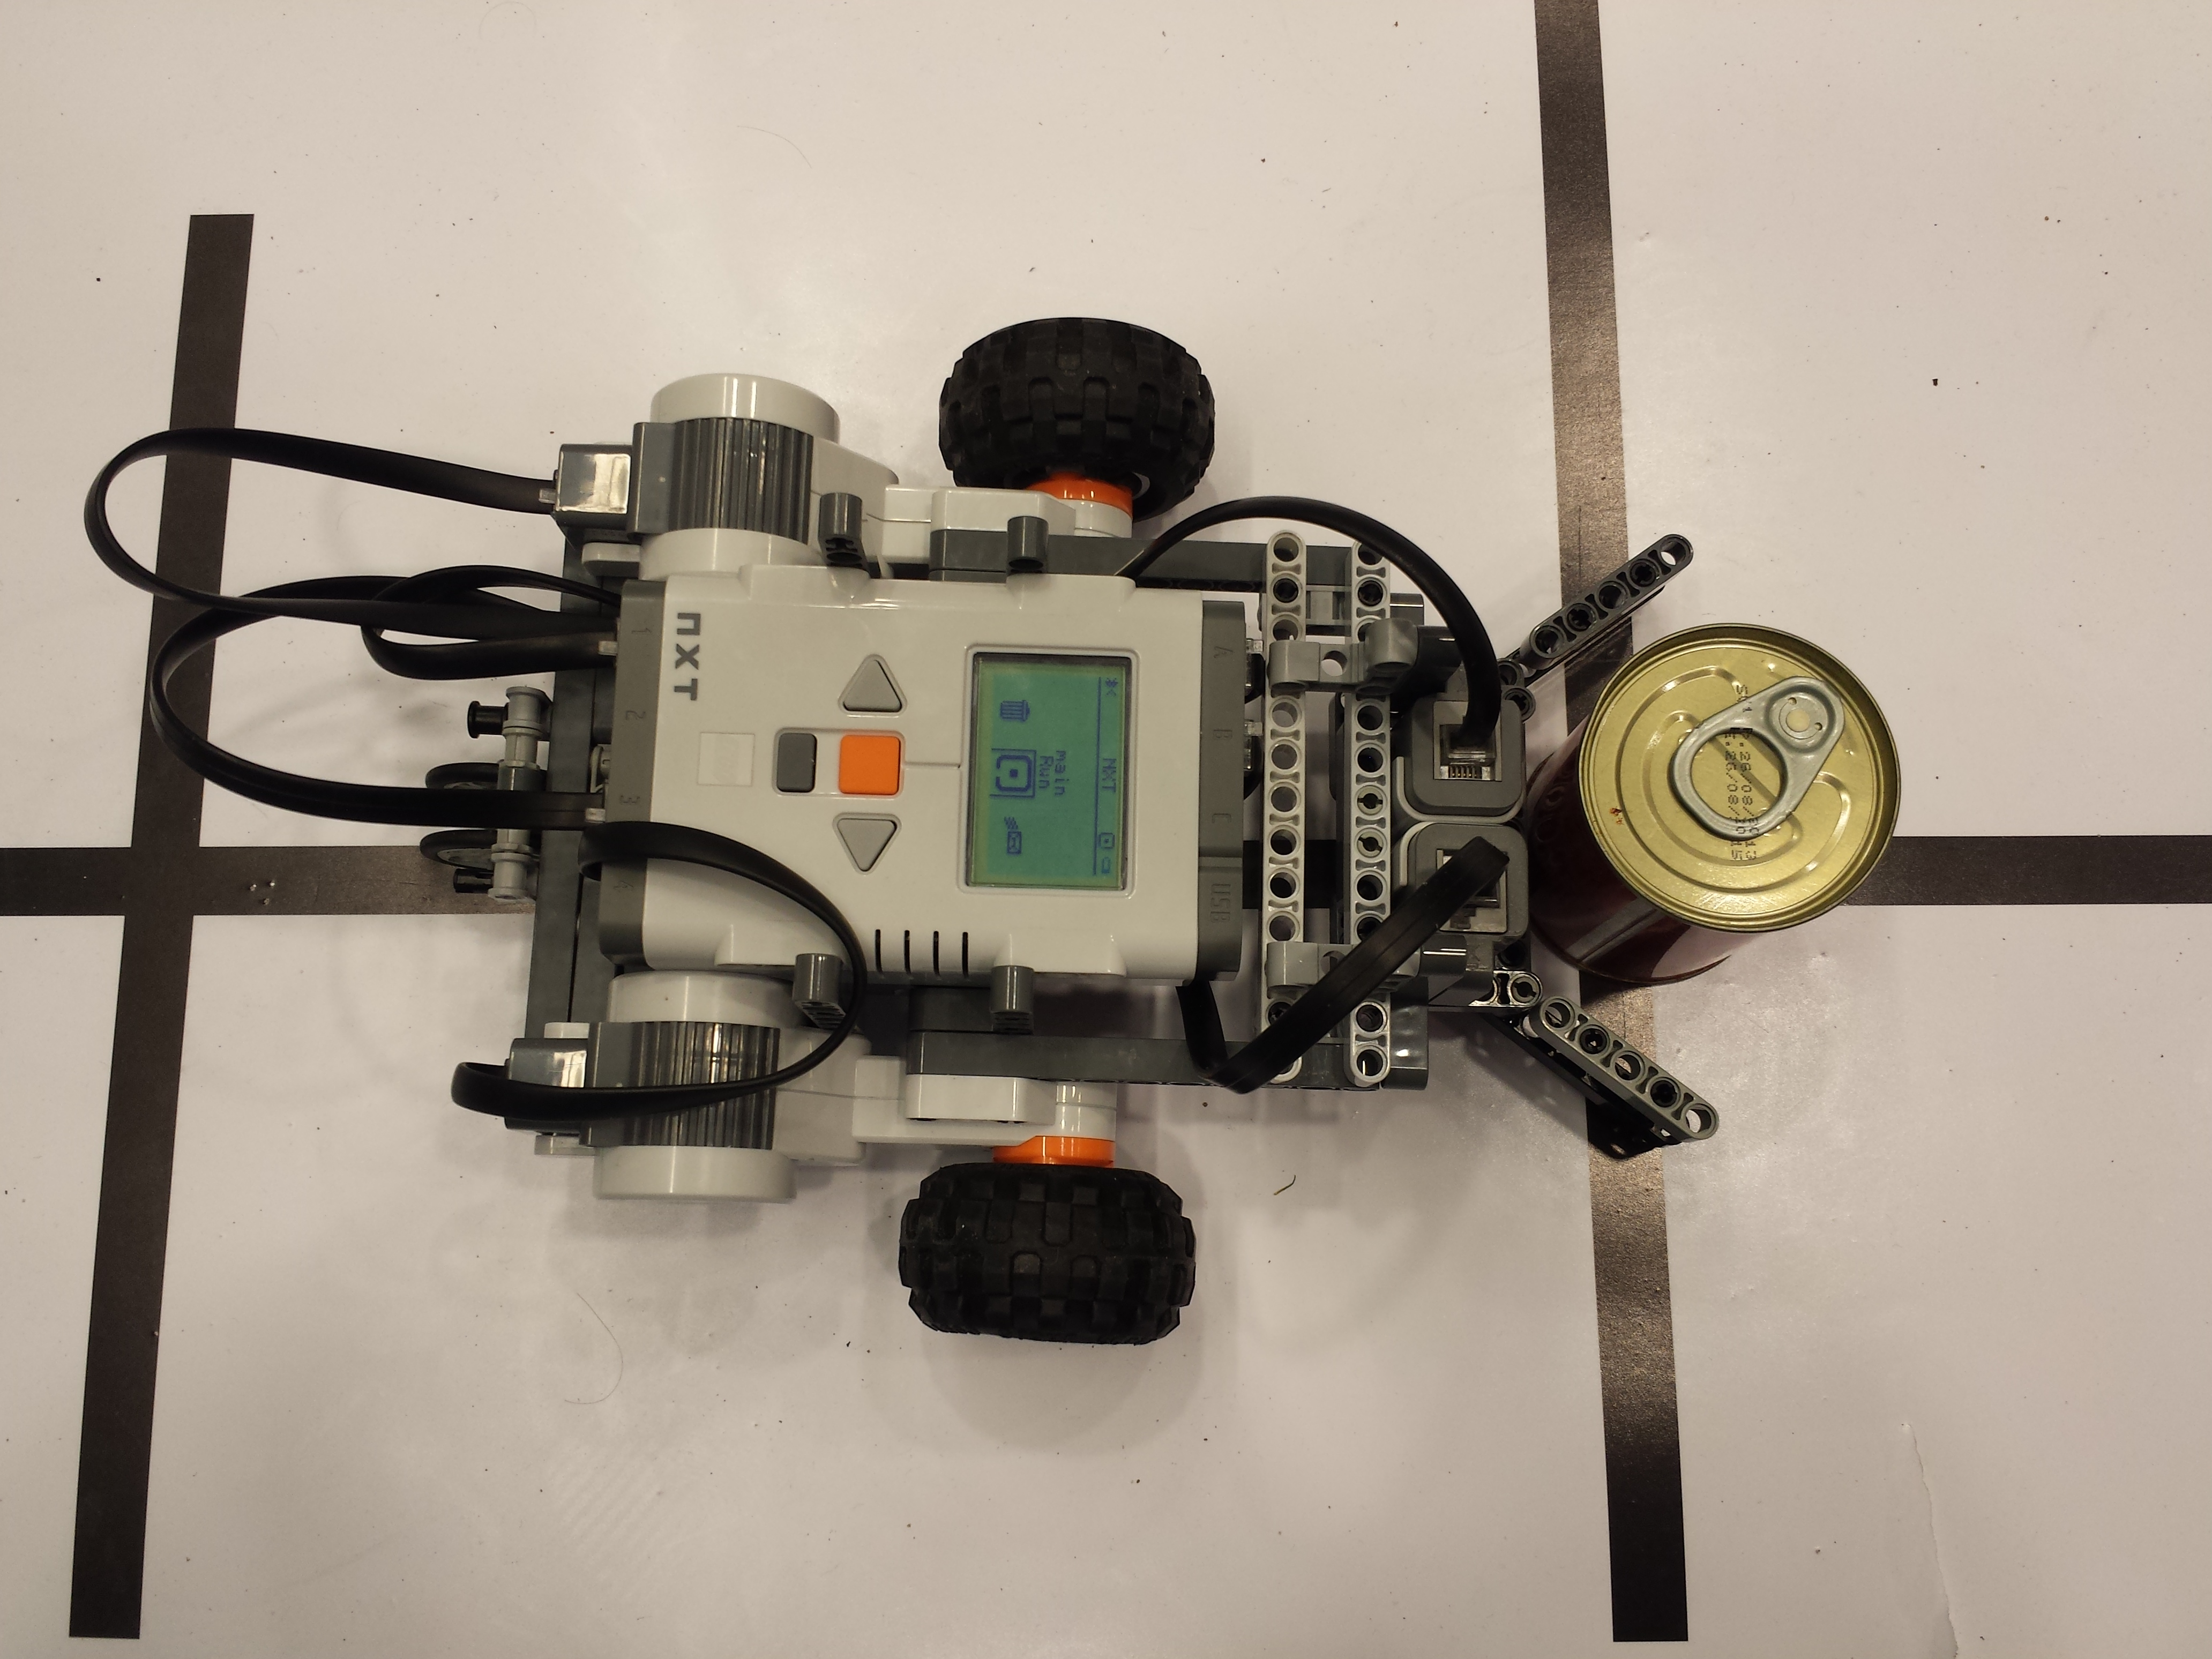
\includegraphics[width=0.34\textwidth]{robot}
 \caption{The Robot prototype}\label{fig:robot}
\end{figure}
\section{Speed and Reliability}
The speed and reliability is determined by the PID coefficients, the default move speed and the number of moves.
An increase of speed will make the system more unstable, risking the robot looses track of the line.
The number of moves can be optimized by the sokoban solver and should thus be optimized.
The sokoban solver finds the optimal solution according to a path cost.
An naive solution will thus calculate the path cost as the number of fields moved.
By measuring the time it takes for each robot move, a more detailed path cost can be calculated.
A detailed path cost will be more expensive on the sokoban solver, both in terms of memory and execution speed.
This is considered irrelevant to the task at hand so this is acceptable.

\section{Documentation of Performance}
The performance of the sokoban solver will be measured in maximum memory consumption and execution speed on several common maps.
To test how the solver handles special situations in the game a series of maps specifically made to provoke the solver will be devised or found from similar projects.

The robots performance should be measured on the timing of the individual robot moves as well as the resulting movement macros generated by the compass function.
The stability should be measured by trying combinations of robot moves that proves to be extra challenging.
Every robot move should be optimized in a way that allows for the fastest execution as a single robot move as well as allows for quickest recovery so a series of moves will not slow down the robot.


% \todo[inline]{Måske en test der omhandler hvor ofte robotten sætter en dåse præcist ovenpå et kryds, og ikke skubber den for langt/stopper for tidligt}
% \todo[inline,author=Nikolaj,color=blue!20]{Sensorne er monteret 8 mm hvor dåsen vil være placeret. Den detekterer et kryds ved starten af en streg, så placeringen vil aldrig være langt fra center af krydset}
\end{document}
